\chapter{Beamtime}

\section{Beamtime}

Throughout the development of the hodoscope many different experiments have been carried out in the lab to gather more data on the performance of the different elements of the hodoscope. Most of these were carried out using radioactive sources or collected data using cosmic rays. Both of these sources are readily available but are either limited by the energy of the source or the rate of the cosmics. To truly test the detectors performance in an environment comparable to which it will be used once installed requires beamtime. There have been 3 beamtests throughout the detectors development, the first carried out at Jefferson Lab and the following two at the Double Annular $\Phi$  Factory for Nice Experiments (DAFNE or DA$\Phi$NE) Beam Test Facility (BTF). Each one was done in conjunction with a prototype of the FT-Cal, simulating their operating environment in CLAS12.

\subsection{First Test: Hall B at JLAB}

The first test used only a single 15 x 15 x 10 mm$^{3}$ tile read out by 2 wavelength shifting fibres. These were set into channels cut into the surface of the tile, rather than inset into holes. The test configuration in Hall B at JLAB is shown in Figure \ref{HallBTestSetup}

\begin{figure}
	\centering
	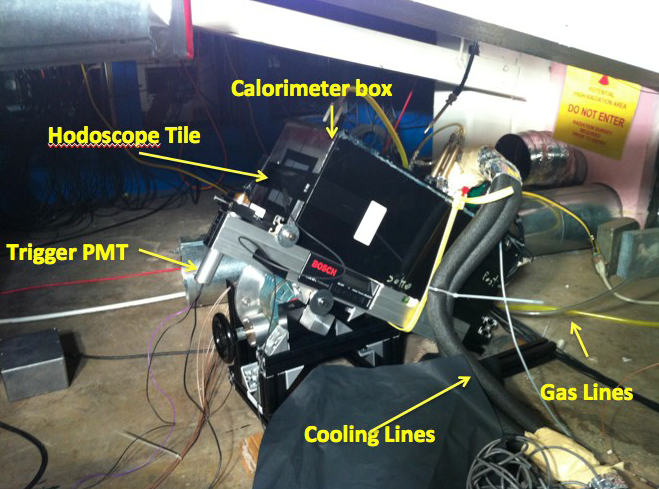
\includegraphics[width=0.7\textwidth]{ImgChap1/firsttest}
	\caption{The set-up for the first beamtest in Hall B.}
	\label{HallBTestSetup}
\end{figure}

The main aim was to provide an initial proof of principle test of the equipment and to provide further information to guide the development of the detector system under beam conditions. The single hodoscope tile was positioned in front of one of the elements of the calorimeter to take coincidence measurements.

The results of the energy deposited in the hodoscope and calorimeter tile can be plotted in 2D to determine the spread of hits measured in the test. An example is shown in Figure \ref{HallBTestResult}, with a clear region of coincident hits measured between the two detector tiles. 

\begin{figure}
	\centering
	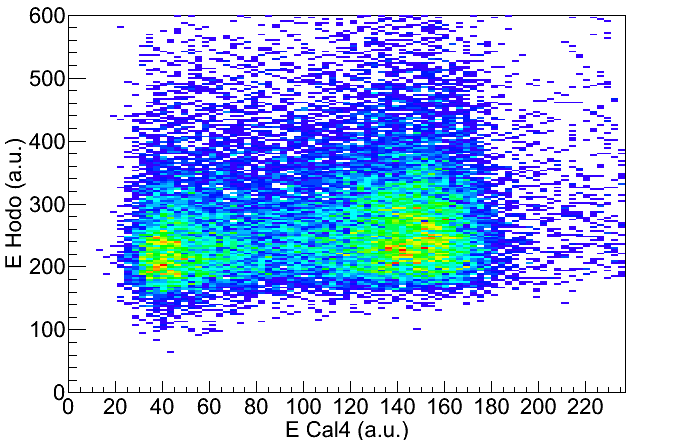
\includegraphics[width=0.9\textwidth]{ImgChap1/HodoTest2}
	\caption{An example of the spread of Energy deposited in the test set-up in Hall B. The energy of hits in the hodoscope vs the calorimeter are shown (terms of the ADC channel). The cluster on the left represents pedestal measurements and the cluster on the right are coincident hits between the two detectors.}
	\label{HallBTestResult}
\end{figure}

This initial test of a simple readout situation was a success and provided plentiful information to improve the design of the detector system. However the light output and isolation of the tiles needed to be improved to reach the design requirement of the system.


\subsection{Second Test: BTF at DA$\Phi$NE}

This following set of beam tests took place at the DA$\Phi$NE $e^{+}e^{-}$ collider siutated at the INFN Frascati National Laboratory, Frascati Italy. This facility primary collides electrons and positrons at a centre of mass energy of 1.02 GeV to produce $\phi$ mesons that primary decay to kaons that are the main focus of the experiments taking place at the accelerator. The leptons are in the facility are first accelerated by a LINAC to 510 MeV before being injected into the accumulator. However when injection is not taking place the beamline can be delivered to a beam test area (BTF). \cite{mazzitelli2003commissioning}. The BTF facility is capable of delivering beam for a wide range of energies and multiplicities and is mainly used for calibration experiments.


\begin{figure}
	\centering
	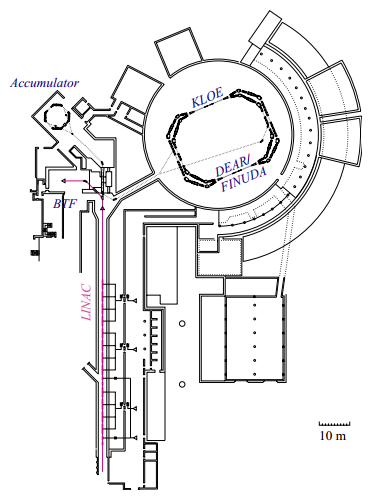
\includegraphics[width=0.7\textwidth]{ImgChap1/BTF}
	\caption{An arial overview of the accelerator facility at DA$\Phi$NE. \cite{mazzitelli2003commissioning}}
	\label{BTF}
\end{figure}

The tests main purpose was to test a range of hodoscope elements at the same time, in coincidence with multiple calorimeter elements. A total of 8 tiles were prepared 4 larger P30 tiles and 4 smaller p15 tiles, with an even split between thick (15mm) and thin (7mm) tiles. The elements prepared used initial designs for reflective materials, optical connections and electronics with 8 hodoscope channels being read out simultaneously.

\begin{figure}
	\centering
	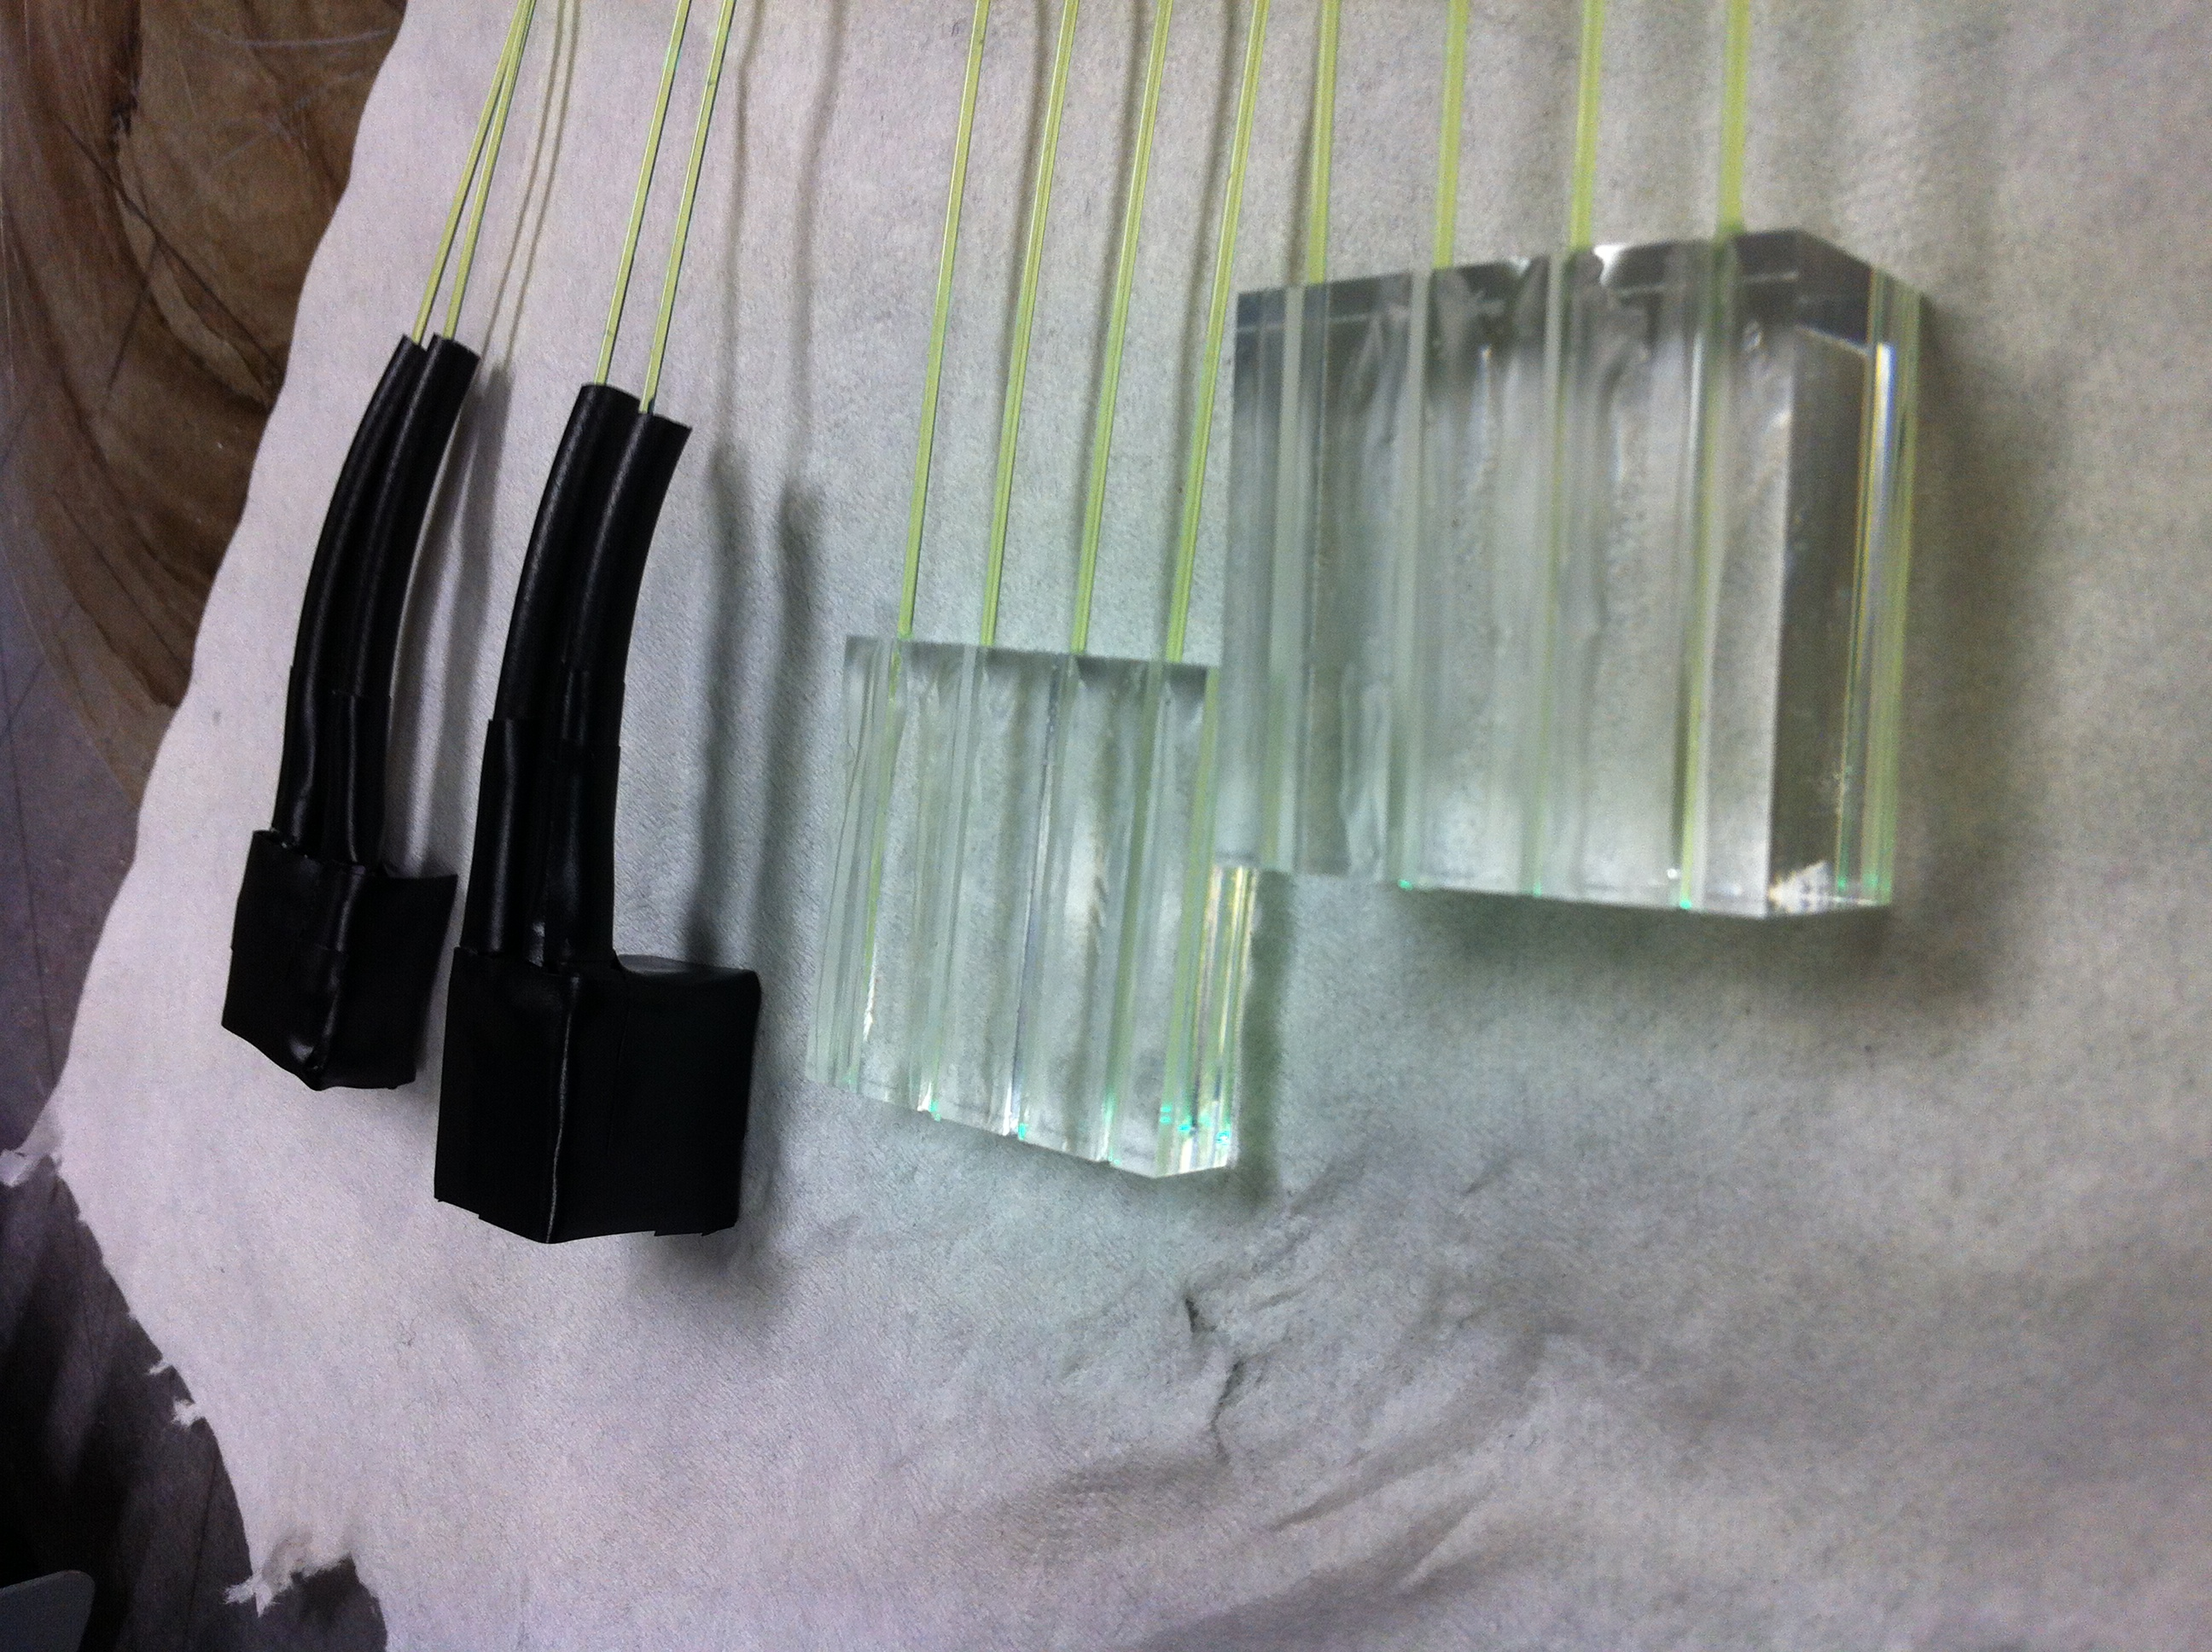
\includegraphics[width=0.7\textwidth]{ImgChap1/frascatitile}
	\caption{Some of the tiles used during the frascati tests. 2 after being wrapped and 2 before.}
	\label{Frascati2Tiles}
\end{figure}

The Tiles used were positioned in 2 layers, with 2 wider p30s and 2 smaller p15 tiles used in each layer,  with the thicker tiles mounted behind the thinner layer. Each tile was aligned with corresponding elements in the prototype calorimeter for coincidence measurements during the experiment. For ease of readout some fibres were connected using shorter ($\sim$ 0.2m) and other longer ($\sim$ 1m) fibres. A simple diagram of the set-up is shown in Figure \ref{Frascati2SetupDiagram}. 

\begin{figure}
	\centering
	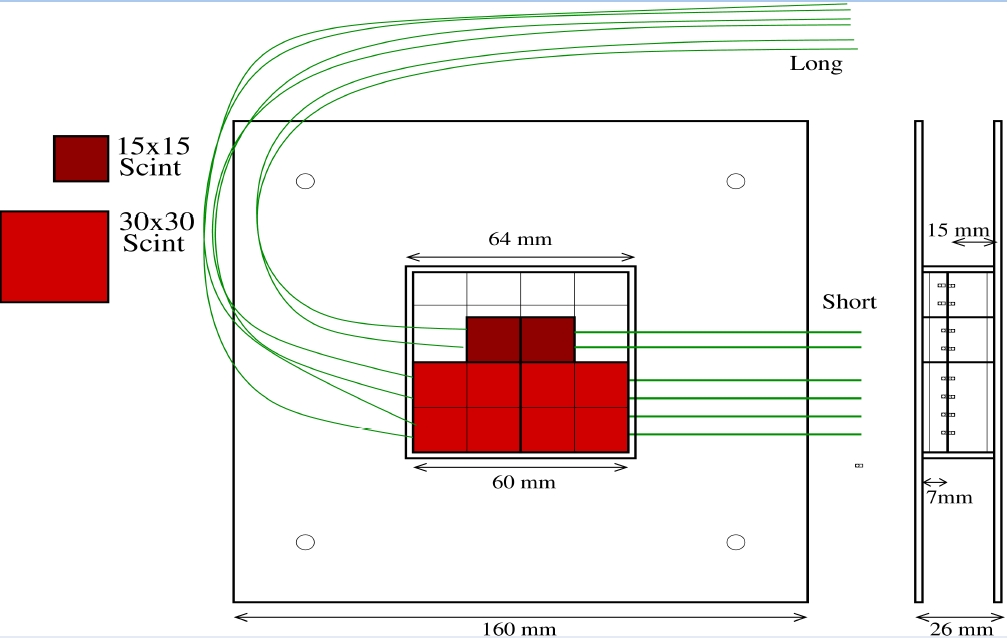
\includegraphics[width=0.7\textwidth]{ImgChap1/frascati1}
	\caption{Schematic set-up for the BTF tile tests. Configuration with the beamline directed into the page with the calorimeter positioned downstream of the prototype hodoscope.}
	\label{Frascati2SetupDiagram}
\end{figure}

The results of the tests were positive successfully taking data from the 8 tiles simultaneously in coincidence with the calorimeter. However there were clear problems with both the overall output of the tiles and the consistency of results between them, an example of these is shown in Figure \ref{Frascati2Results1}. 

\begin{figure}
	\centering
	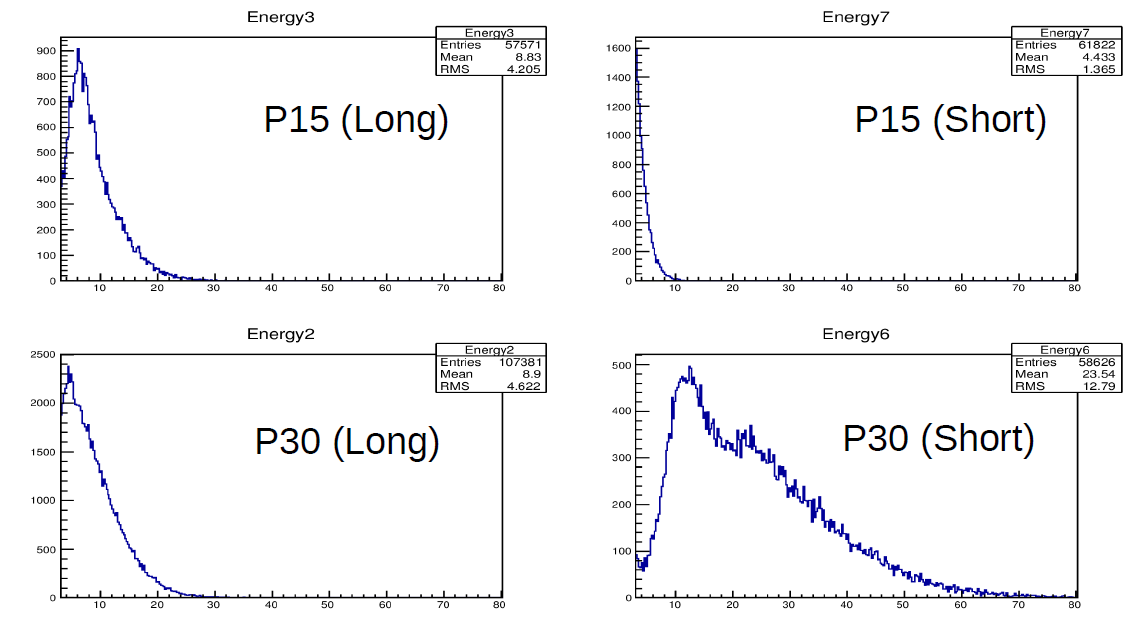
\includegraphics[width=0.9\textwidth]{ImgChap1/frascatiresults1}
	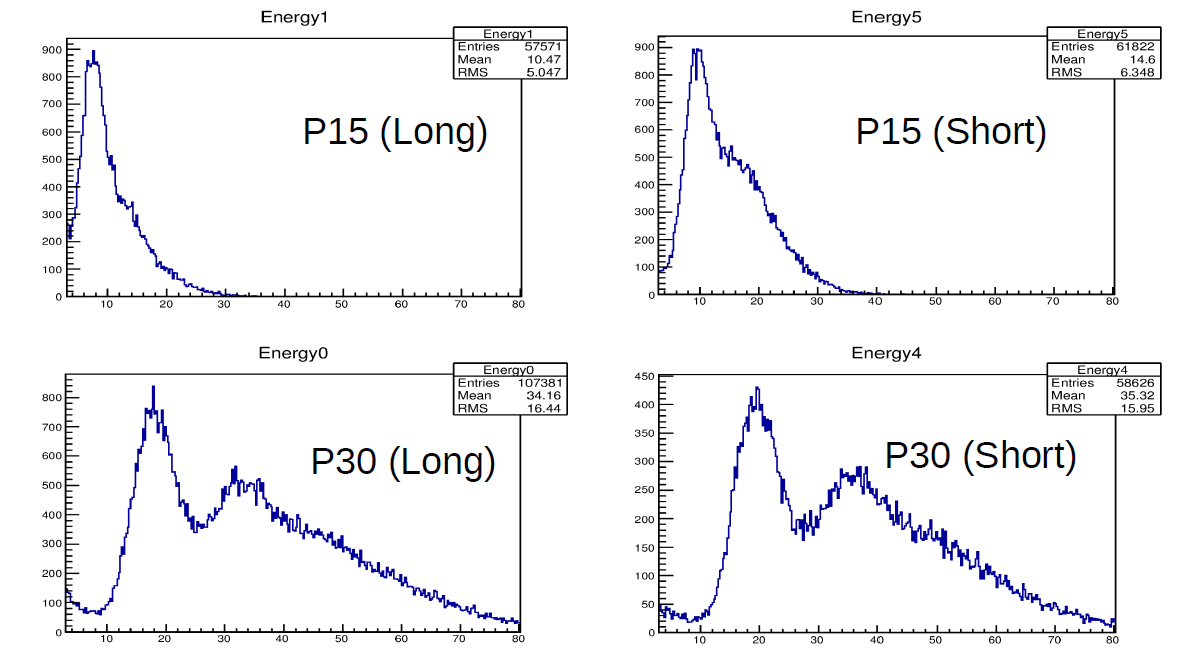
\includegraphics[width=0.9\textwidth]{ImgChap1/frascatiresults2}
	\caption{Sample results from the first tests run at the BTF (x-axis units are photoelectrons). Results are shown for the 4 thin tiles (Top four frames)} and the 4 thick tiles (Bottom four frames). Results for both single and double electron bunches can be clearly seen, most obviously for the P30 Thick tiles. 
	\label{Frascati2Results1}
\end{figure}

The results obtained are well below the expectations from simulations, however during the tests it was found that some of the tiles experienced both poor and inconsistent optical connections both Tile$\rightarrow$Fibre and Fibre$\rightarrow$SiPM. Attempts were made to adjust these during the tests but more fundamental adjustments to the design were required to resolve some of these problems. The strongest performing tiles were the P30 thick tiles, which averaged $\sim$18 photoelectrons for a MIP. 




\begin{figure}
	\centering
	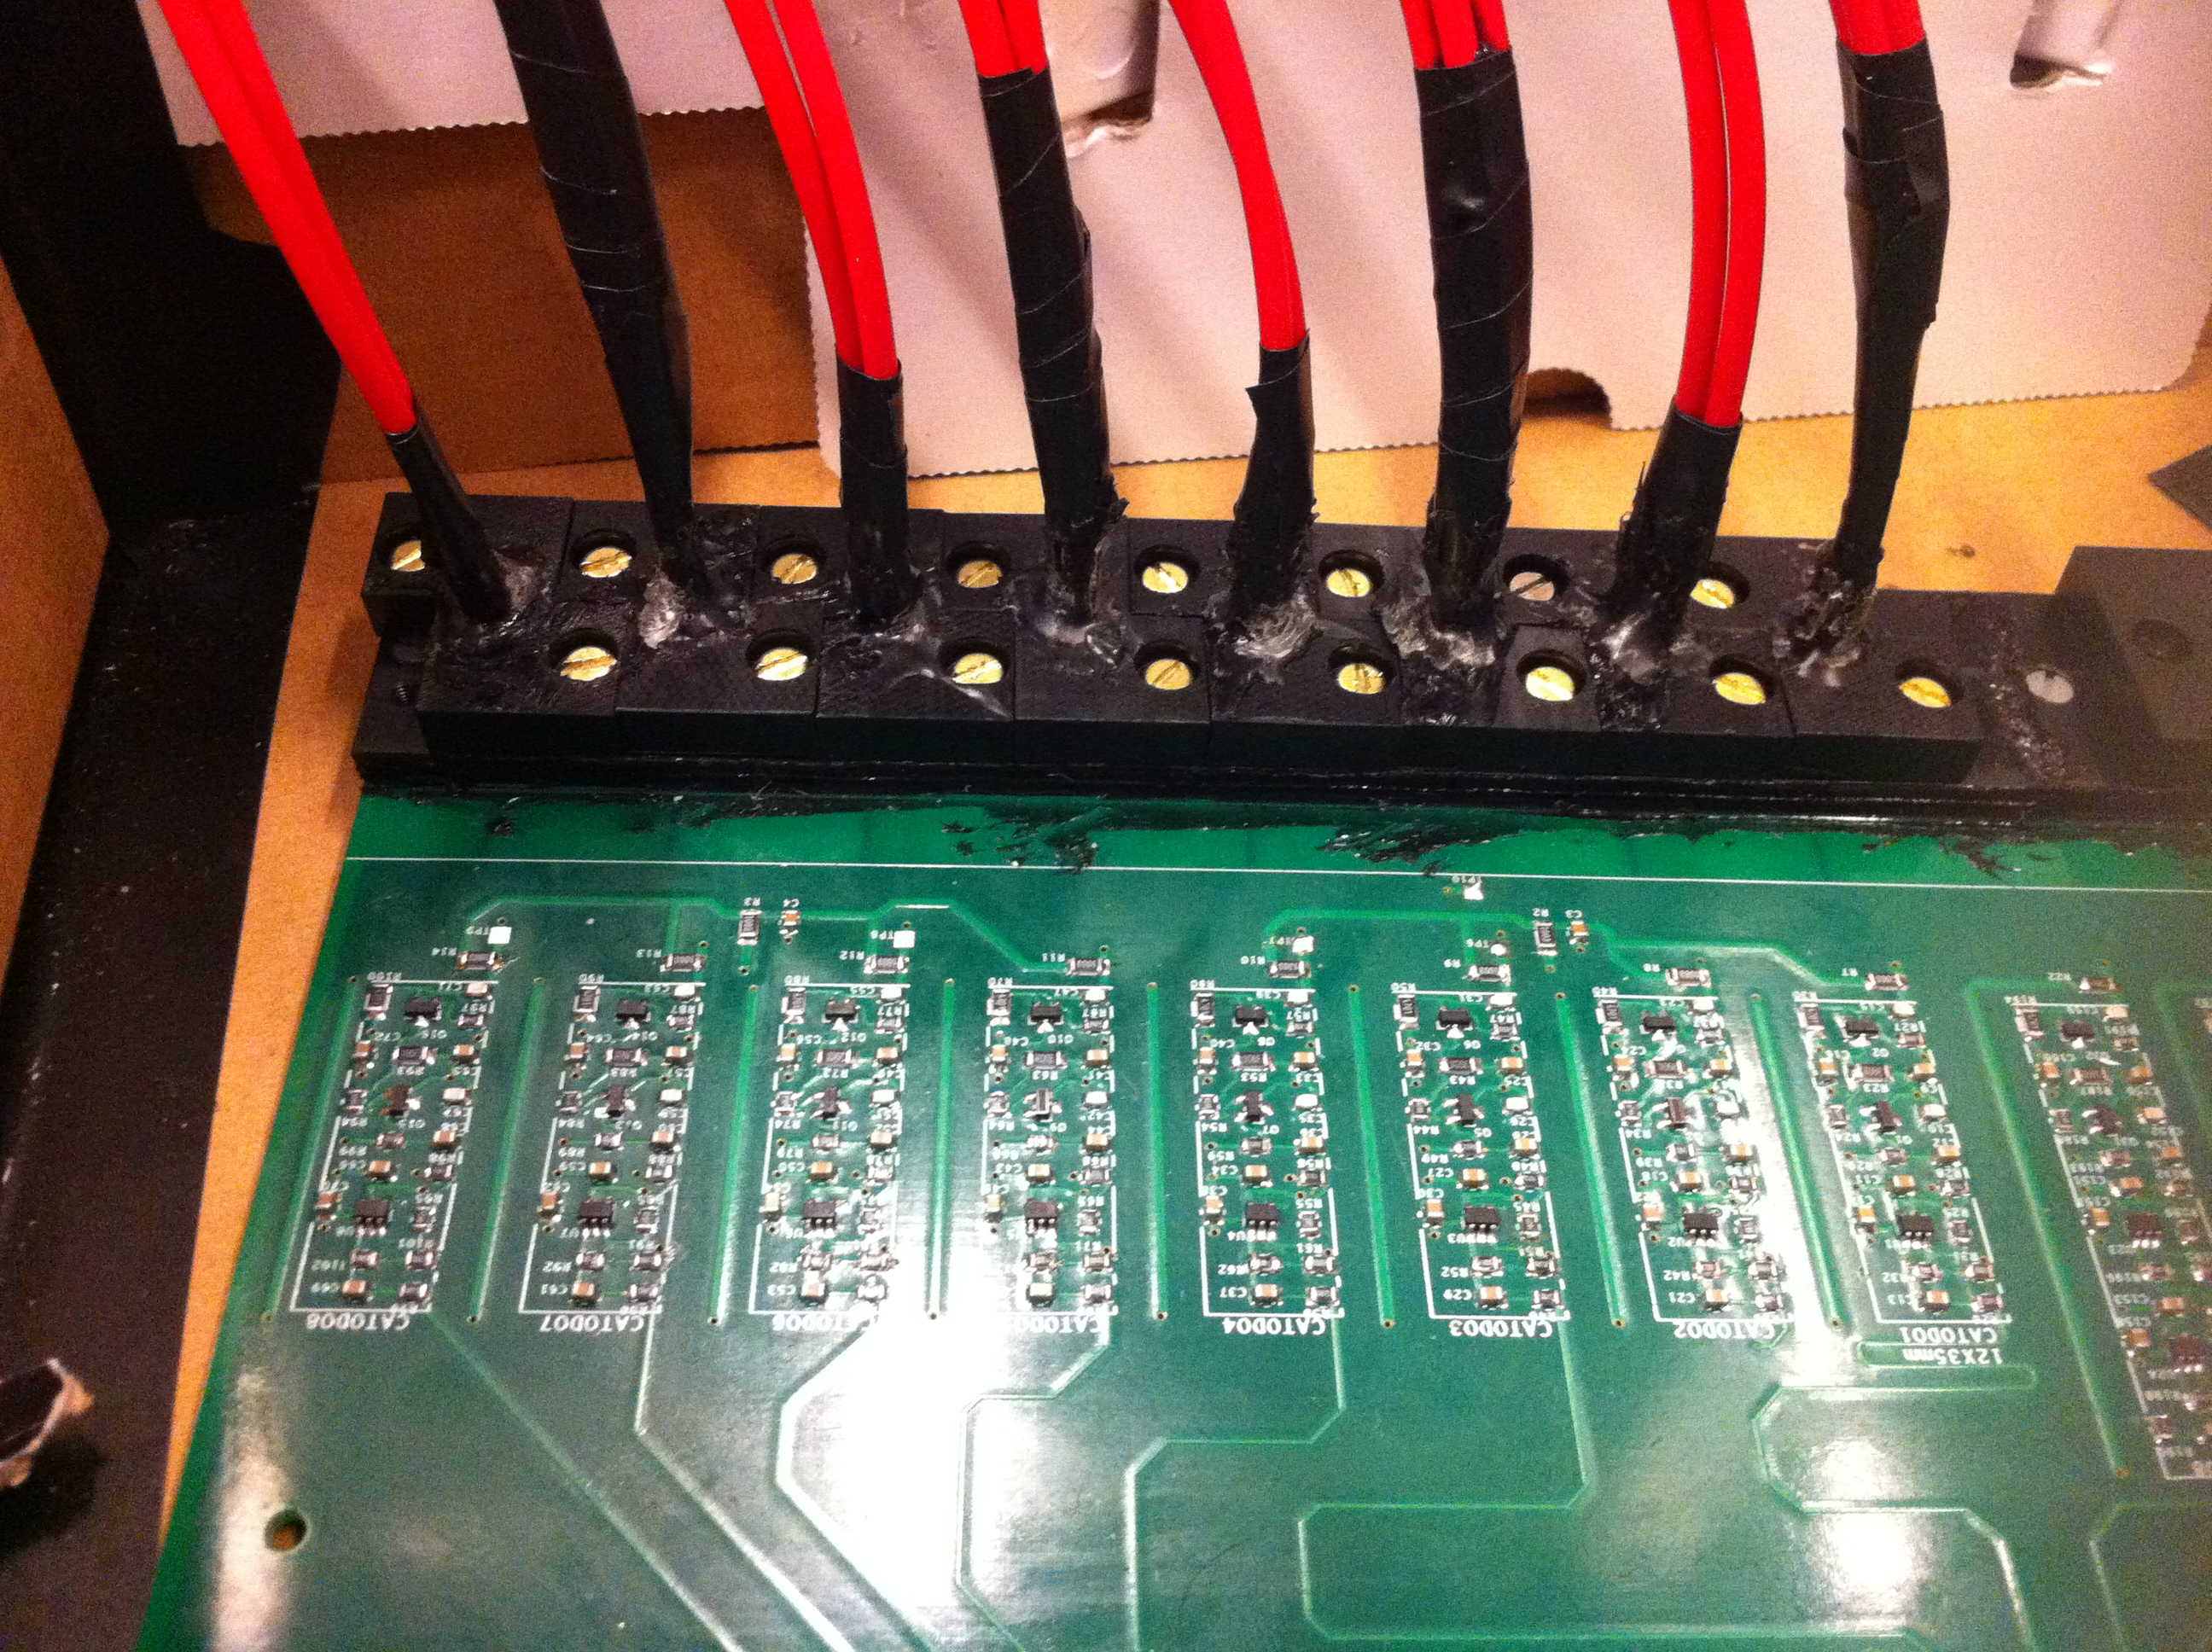
\includegraphics[width=0.7\textwidth]{ImgChap1/holderboard}
	\caption{A photograph of 8 fibre channels attached to a prototype board supporting the SiPMs.}
	\label{Frascati2SetupDiagram}
\end{figure}




\subsection{Third Test: BTF at DA$\Phi$NE}

A second set of beam studies at DA$\Phi$NE was carried out on prototype hodoscope detector in November 2012. This set of tests used a similar configuration to those utilised at the previous test, but the focus was put onto improving the optical output of the tiles demonstrating the viability of the detector design. A variety of new tiles were tested, including some previously trialled at the previous round of testing. Improvements were made to the reflective wrapping of the tiles and optical isolation of the elements. However the most significant progress was made in the quality of the optical connections tiles-fibres and fibres-SiPMs. Where each group of fibres was glued into a SiPM connector, before being polished using a series of refining grades of optical sandpaper, to ensure a clean optical connection to the SiPMs.

%Tiles used in each round of testing were positioned in 2 layers, with 2 wider p30s and 2 smaller p15 tiles used in each layer. The electronics were positioned to one side of the detector system, outside of the beamline, which necessitated the fibres from some tiles to be longer than others, see Figure \ref{Frascati2SetupDiagram}. 

\begin{figure}
	\centering
	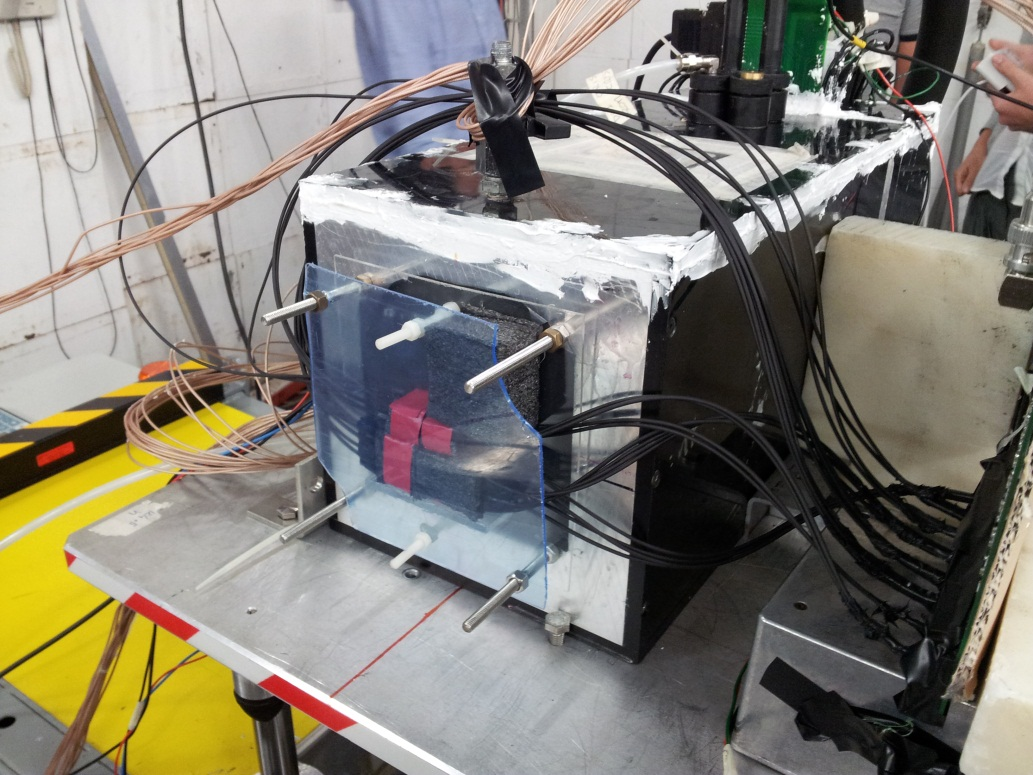
\includegraphics[width=0.7\textwidth]{ImgChap1/frascatiphoto}
	\caption{Photograph of the prototype configuration in situ in frascati, prior to the start of the beamtime.}
	\label{Frascati2SetupPhoto}
\end{figure}

\begin{table}\centering
	\renewcommand{\arraystretch}{1.3}
	\begin{tabular}{ @{}l  c  c  c  c@{}} 
		\toprule
		Tile & Thickness &Fibre Length & Source & Photons \\
		& {\small [mm]}& {\small [m]} & & \\
		\midrule
		P30Thn & 7 & 0.2 & Eljen* & 37 \\
		P30Thn & 7 & 1.0 & Eljen* & 28 \\
		P15Thn & 7 & 0.2 & Eljen* & 23 \\
		P15Thn & 7 & 1.0 & Elgen* & 19 \\
		P30Thk & 15 & 0.2 & NE & 78 \\
		P30Thk & 15 & 1.0 & NE & 35 \\
		P15Thk & 15 & 0.2 & Eljen & 29 \\
		P15Thk & 15 & 1.0 & Eljen & 23 \\
		P30Thk & 15 & 0.2 & Elgen & 46 \\
		\bottomrule
	\end{tabular}
	\caption{Summary of tile performance during the second set of tests at BTF. Tiles marked with a * were also tested at the previous beamtime at BTF, but now with upgraded fibre$\rightarrow$SiPM connections.}
	\label{Frascati2ResultsTable}
\end{table}

Nine different tiles were tested during the beamtime, with the P30Thk tiles being switched between runs. The overall performance of the tiles increased significantly from the results obtained at the previous test, with the best performing tile peaking at just under 80 photoelectrons, shown in Figure \ref{Frascati2Results} However the results were still not consistent across size, thickness and fibre length and the majority of tiles were still performing below the potential indicated by simulations. This set of results was promising and demonstrated the tiles can reach the level of output required for suitable timing resolution of the detector. Further studies were needed to raise the number of photons reaching the SiPMs and improve the consistency of tile performance to allow every detector element to reach the same peak performance. Figure \ref{Frascati2Results} show of plot of the best performing tile in the tests.

\begin{figure}
	\centering
	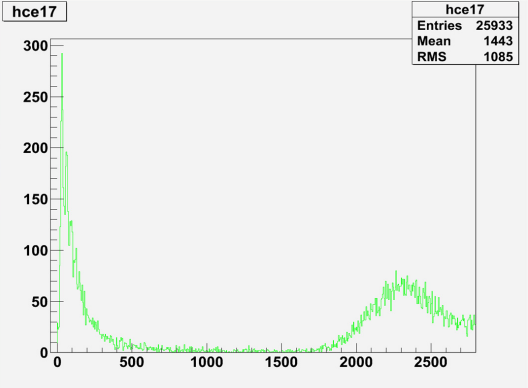
\includegraphics[width=0.7\textwidth]{ImgChap1/frascati2results}
	\caption{A plot of the strongest performning tile from the second set of tests at BTF. The MIP landau is well seperated from the thermal noise across almost the full range of the ADC, peaking at an energy equivalent to just below 80 photoelectrons.}
	\label{Frascati2Results}
\end{figure}   